% !TeX spellcheck = en_US

\section{Approach} % Method
\begin{figure}
	\centering
	% !TeX spellcheck = en_US
\tikzset{
	operation/.style={fill=white, text centered},
	block/.style = {operation, rectangle, draw, text width=0.175\textwidth, minimum height=1cm},
}
\begin{tikzpicture}[node distance = 1cm and 1.75cm]
	\node (image)           [block] {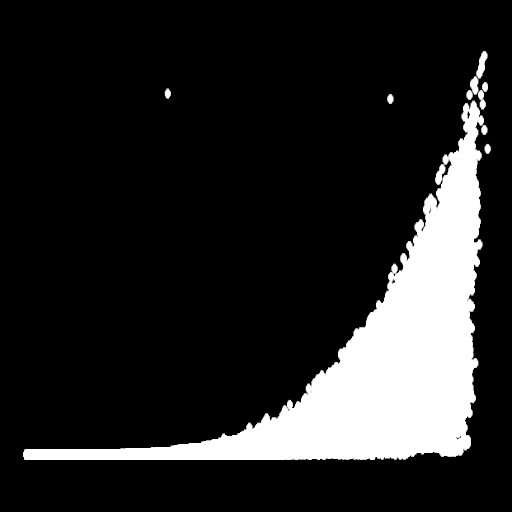
\includegraphics[width=\textwidth]{figures/input.jpg} Image \image};
	\node (aperture)        [block, right = of image] {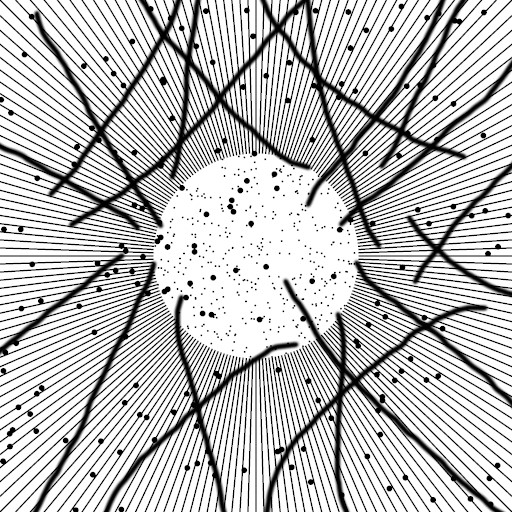
\includegraphics[width=\textwidth]{figures/aperture.jpg} Aperture \aperture};
	\node (blobMask)        [block, below = of image] {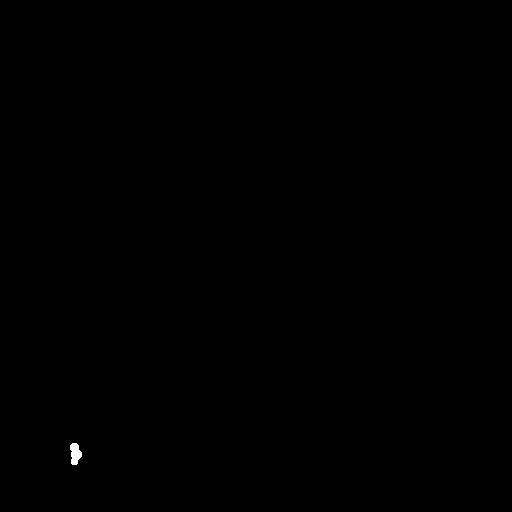
\includegraphics[width=\textwidth]{figures/blobMask.jpg} Blob mask \blobmask};
	\node (tonemappedImage) [block, left = of blobMask] {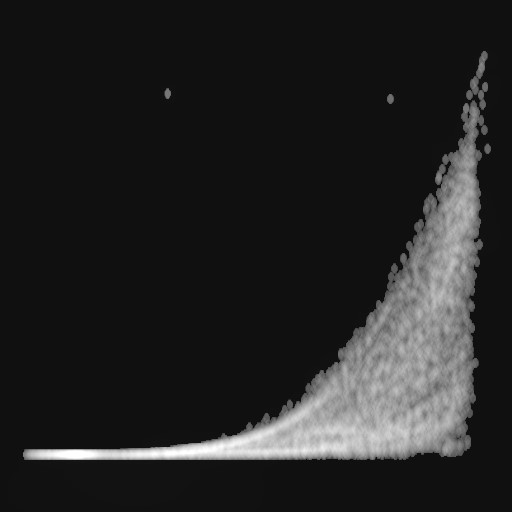
\includegraphics[width=\textwidth]{figures/tonemappedImage.jpg} Tone mapped image \tonemappedimage};
	\node (overlay)         [block, below = of blobMask] {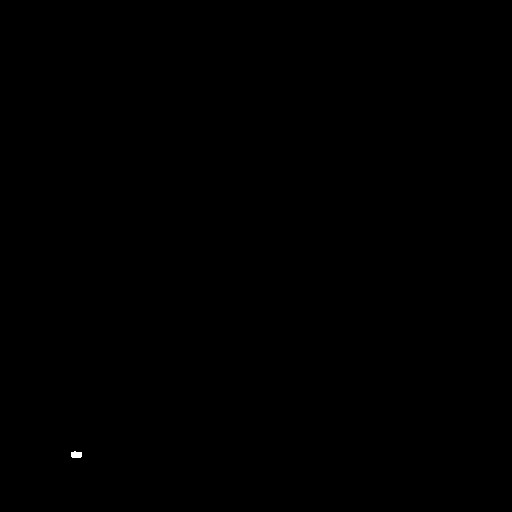
\includegraphics[width=\textwidth]{figures/overlay.jpg} Bright pixels \overlay};
	\node (psf)             [block, right = of overlay] {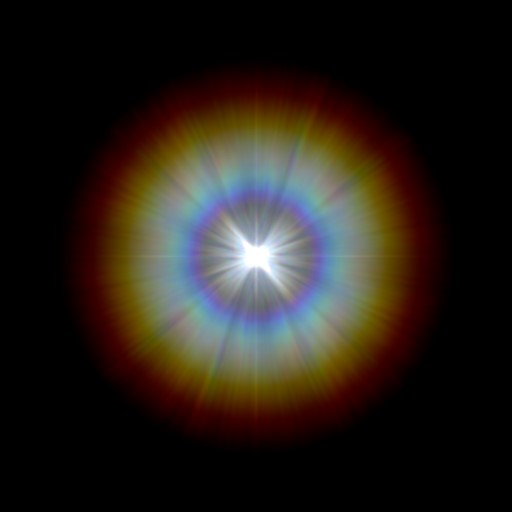
\includegraphics[width=\textwidth]{figures/psf.jpg} Glare filter \psf};
	\node (glareOverlay)    [block, below = of overlay] {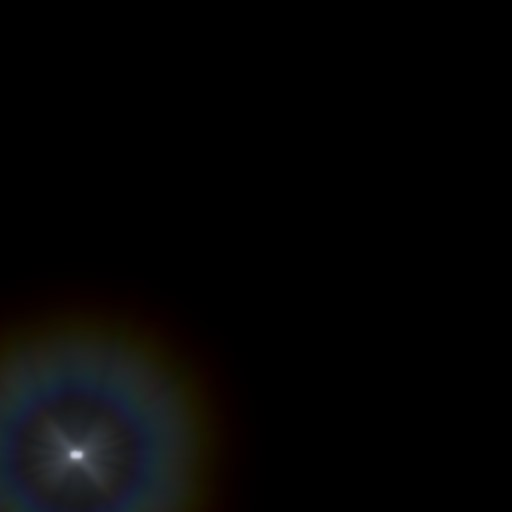
\includegraphics[width=\textwidth]{figures/glareOverlay.jpg} Glare overlay \glareoverlay};
	\node (output)          [block, below = of glareOverlay] {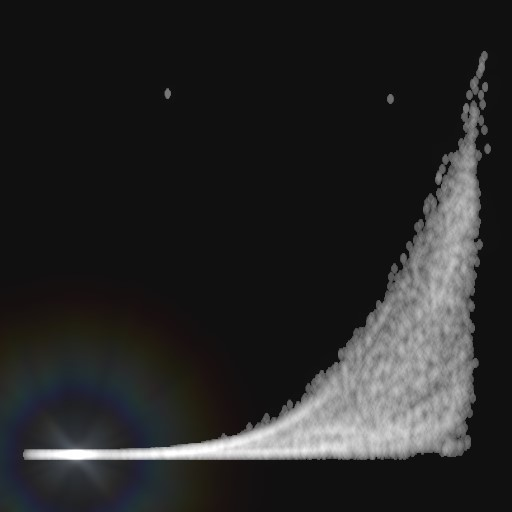
\includegraphics[width=\textwidth]{figures/output.jpg} Tone mapped and glared image \finalimage};
	
	\draw[white] (image) -- node(dummy){} (aperture);
	
	\draw[->] (image) -- node(detection)[operation]{Blob detection} (blobMask);
	\draw[->] (image) -| node[operation]{Tone mapping} (tonemappedImage);
	\draw[->] (aperture) -- node[operation, text width = 0.175\textwidth]{Diffraction approximation} (psf);
	
	\draw[->] (blobMask) -- node(masking)[operation]{Masking} (overlay);
	\draw     (tonemappedImage) |- (masking);
	\draw     (image) -- (dummy.center) |- (masking);
	
	\draw[->] (overlay) -- node(convolution)[operation]{Convolution} (glareOverlay);
	\draw     (psf) |- (convolution);
	
	\draw[->] (glareOverlay) -- node(adding)[operation]{Blending} (output);
	\draw     (tonemappedImage) |- (adding);
\end{tikzpicture}
	\caption{Pipeline.}
	\label{fig:pipeline}
\end{figure}

We combine tone mapping with glare simulation for a automated visualization of images.
The pipeline of our approach can be seen in \Cref{fig:pipeline}.
Results of steps are shown in boxes together with the image for one example.
The image \image{} and aperture \aperture{} are the inputs of the pipeline and the tone mapped and glared image \finalimage{} is the output.
Steps are shown as text connected to the respective output of the step (below) and one or more inputs to the step (above).
In the following the steps of our approach are described.

\paragraph{Tone Mapping}
The tone mapping operator of \citeauthor{Mantiuk2006}~\cite{Mantiuk2006} was used because it is based on the human perception of contrast in images.
This makes this tone mapping operator suitable for visualization of density plots, as it %TODO

We used the \term{contrast mapping} approach for modifying the contrast response, as %TODO
This approach has one parameter: A value between 0 and 1.
Higher values %TODO
lower values %TODO
\Citeauthor{Mantiuk2006} suggest a value between.

In this approach contrast is computed for one neighbor in \xdir{} and \ydirection{}.
The contrast $\contrast_x^k$ is the contrast of a pixel and the next pixel in \xdirection{} (if there is one),
otherwise it is zero.
$\contrast_y^k$ is is defined analogously for the \ydirection{}.
$G_x^k$ and $G_y^k$ are computed for all pixels on all levels of the Gaussian pyramid (see \Cref{eq:contrast}).

The same neighborhood has to be considered in \Cref{eq:optimization-problem} for solving the optimization problem.

\paragraph{Diffraction Approximation}
For the glare simulation we used an approach based on the work of \citeauthor{Kakimoto2004}~\cite{Kakimoto2004} and \citeauthor{Ritschel2009}~\cite{Ritschel2009}.
For this only the \Cref{eq:fresnel} or \Cref{eq:fraunhofer} and \Cref{eq:spectral-psf} have to be implemented.
As first approach only the Fraunhofer diffraction and a static aperture loaded from an image file are used.
It could be expanded to use the Fresnel diffraction and a dynamic simulation of the human eye.
% franhufer diffraction, static input, no simulation of human eye

As the constructed glare filter should be only applied to bright pixels.
We use an automated blob detection to find these.

\paragraph{Blob Detection}
Using the normalized Laplacian response \normlaplacescalespace{}, blobs in scalar images can be detected.
We use the luminance image \luminance{} of the original image \image{} for the blob detection.
Detecting all local extrema in \normlaplacescalespace{} leads to blobs, of which many only cause a small response.

For discrete images, the scale\hyp{}space \scalespace{} has to be discretized.
The spatial dimensions are discretized like the original image and sampling in the scale dimension should be linear for fine scales and exponential for coarser scales \cite[see][Footnote 2]{Lindeberg1998}.
The chosen scales $\sigma_i$
\begin{align}
	\sigma_i &= \sqrt[4]{2^i}
\end{align} 
satisfy this.
%TODO: FIX
% http://www.wolframalpha.com/input/?i=linear+regression+%7B%7B0,+1%7D,+%7B1,+1.18920712%7D,+%7B2,+1.18920712%5E2%7D,+%7B3,+1.18920712%5E3%7D,+%7B4,+1.18920712%5E4%7D%7D
% On small scales (0,1,2,3,4) this a linear function can fit the data with a coefficient of SOMETHING with 0.9897
% while the overall behavior is exponential.
%
% The maximum scale is chosen in a way that the radius corresponding to the scale is the first one so a circle's diameter is above 20% of the image
%
%
%

Local extrema in the discretized scale\hyp{}space can be found by comparing a value to its 26 neighbors:
eight on the same scale, nine on the next lower scale, and nine on the next higher scale.
On boundaries of \scalespace{} less than 26 neighbors exist and have to be compared.
To not take the sign of \normlaplacescalespace{} into account, absolute values are used and the local maximum has to be found \cite{Lindeberg1998}.

Like \citeauthor{Lindeberg1998}~\cite{Lindeberg1998}, we threshold and draw circles for blobs.
Local extrema with a value of $\normlaplacescalespace{}$ smaller than the threshold are ignored, while the remaining ones are classified as blobs.
For a local extremum at position $(\vector{x}_i, \sigma_j)$, a solid circle with radius $\sqrt{2} \cdot \sigma_j$ and center $\vector{x}_i$ will be drawn on the the blob mask \blobmask{}.

This radius is used so the zero\hyp{}crossings of the Laplacian of the Gaussian align with a circle of radius $r$.
The Laplacian of the Gaussian 
\begin{align}
	\laplace \gaussian(x, y, \sigma) &= \frac{x^2 + y^2 -2\sigma^2}{2 \pi \sigma^6} \exp\left(- \frac{x^2 + y^2}{2 \sigma^2} \right)
\end{align} 
has zero\hyp{}crossings when $x^2 + y^2$ equals $2\sigma^2$.
Let the circle (without loss of generality) be centered around $(0, 0)$, so $x^2 + y^2$ equals $r^2$.
Then the radius is $\sqrt{2}$ times the scale it was detected on.

Using this relation between scales and radii of blobs, a maximum scale can be defined.
In this approach the maximum scale is set to the first scale, on which a blob's diameter exceeds 20\% of the minimum of image with and height.

%\begin{algorithm}
%	\begin{algorithmic}[1]
%		\Function{IsExtremum}{$\scalespace, \vector{x}, \sigma_i$}
%		\State $(x, y) \gets \vector{x}$
%		\ForAll{$a \in \{x-1, x, x+1\}$}
%			\ForAll{$b \in \{y-1, y, y+1\}$}
%				\ForAll{$c \in \{\sigma_{i-1}, \sigma_i, \sigma_{i+1}\}$}
%					\If{$(a, b, c) \neq (x, y, \sigma_i) \wedge \abs{S(a, b, c)} \geq \abs{S(x, y, \sigma_i)}$}
%						\State \Return \texttt{false}
%					\EndIf
%				\EndFor
%			\EndFor
%		\EndFor
%		\State \Return \texttt{true}
%		\EndFunction
%		\Statex
%		\Function{DrawCircle}{$\blobmask, \vector{x}, r$}
%		\State $(x, y) \gets \vector{x}$
%		\For{a}{x-r}{x+r}
%			\For{b}{y-r}{y+r}
%				\If{$(a-x)^2 + (b-y)^2 \leq r^2$}
%					\State $\blobmask(a, b) \gets 1$
%				\EndIf
%			\EndFor
%		\EndFor
%		\EndFunction
%		\Statex
%		\Procedure{BlobDetection}{$\scalespace, \blobthreshold$}
%		\For{i}{0}{\numscales-1}
%			\ForAll{$\vector{x} \in D$}
%				\If{$\Call{IsExtremum}{\scalespace, \vector{x},  \sigma_i} \wedge \abs{S(\vector{x}, \sigma_i)} \geq \blobthreshold$}
%					\State \Call{DrawCircle}{$\blobmask, \vector{x}, \sqrt{2} \cdot \sigma_i$}
%				\EndIf
%			\EndFor
%		\EndFor
%		\EndProcedure
%	\end{algorithmic}
%	\caption{Blob detection}\label{alg:blob-detection}
%\end{algorithm}

\paragraph{Masking}
This blob mask is them used to mask the tone mapped image \tonemappedimage{}.
To only choose the brightest blobs, we also add a brightness threshold to the masking.
The overlay of bright pixels \overlay{} consists of all pixels, where the pixel is within the blob mask and the luminance of the pixel in the original image is above the brightness threshold.
The value of a pixel of \overlay{} is then set to either the color of the tone mapped image at this position or to black.

\begin{algorithm}
	\begin{algorithmic}[1]
		\Procedure{Masking}{$\luminance, \tonemappedimage, \blobmask, \lightthreshold$}
		\ForAll{$\vector{x} \in D$}
			\If{$\blobmask(\vector{x}) > 0 \wedge L(\vector{x}) \geq \lightthreshold$}
				\State $\overlay(\vector{x}) \gets \tonemappedimage(\vector{x})$
			\Else
				\State $\overlay(\vector{x}) \gets 0$
			\EndIf
		\EndFor
		\EndProcedure
	\end{algorithmic}
	\caption{Masking}\label{alg:masking}
\end{algorithm}

\paragraph{Convolution}
The glare filter \psf{} has to be convolved with only the bright pixels \overlay{}.
The convolution theorem can be used to implement the convolution efficiently using two Fourier transforms and an inverse Fourier transform.
\begin{align}
	\glareoverlay (\vector{x}) &= \overlay(\vector{x}) * \psf (\vector{x}) \\
	&= \mathcal{F}^{-1} \left[ \mathcal{F}[\overlay(\vector{x})](\vector{u}) \cdot \mathcal{F}[\psf(\vector{x})](\vector{u}) \right] (\vector{x})
\end{align}

\paragraph{Blending}
The tone mapped image \tonemappedimage{} and the glare overlay \glareoverlay{} have to be combined to get the final image \finalimage{}.
This is done with additive blending.
To add more flexibility, an additional parameter is available to multiply the glare overlay by a constant factor before blending.
This can be used to increase or decrease the intensity of the glare. % default 100%
Leading to the the final image
\begin{align}
	\finalimage(\vector{x}) &= \tonemappedimage(\vector{x}) + \parameterblending \cdot \glareoverlay(\vector{x})
	\intertext{or in the default case with $\parameterblending = 1$}
	\finalimage(\vector{x}) &= \tonemappedimage(\vector{x}) + \glareoverlay(\vector{x})\text{.} \nonumber
\end{align}

\paragraph{Parameters}
Overall our approach leaves four parameters for a user to fine-tune the resulting image.
The steps \step{tone mapping}, \step{blob detection}, \step{masking} and \step{additive blending} all include one parameter each.

\section{Implementation}
The tool was implemented using \Cpp{} and \DirectX{}.

\subsection{Data Structures} % TODO: change
All internal images are stored in \SI{32}{\bit} floating point textures.
The used textures have either a single channel or four channels\footnote{Three-channel \SI{32}{\bit} floating point textures cannot be bound as \code{RenderTargerView}s or as \code{UnorderedAccessView}s.}.

Wrapper structures are used for easier texture management.
The structures keep track of the texture format, with, and height.
There are different wrappers, depending whether the texture should be used as a render target, a resource in a shader, or both.
The last type is used mostly for all algorithms here.
It manages pointers to the texture, an optimal depth buffer, and different views for the texture.
The structure holds one pointer to a \code{RenderTargetView}, a \code{ShaderResourceView}, and an \code{UnorderedAccessView} for the texture and a \code{DepthStencilView} for the depth buffer.

The steps done to generate the final image can be seen in \Cref{fig:pipeline}.
Most steps (tone mapping, blob detection, masking, blending) depend on parameters.
To save computation time when any parameter is changed, some intermediate results are saved to textures, so some steps do not have to be redone.

The intermediate results can be displayed and saved to files.

The \citefield{DirectXTex}{title} library~\cite{DirectXTex} is used to load and store image files.
It supports various file formats for loading and saving file like RGBE, TIFF, DDS, or JPG.



\Computeshader{}s were implemented for the various operations on images.
This includes basic arithmetic operation like adding images or multiplying images with a constant value.
Other 

% preprocessing
% min, max, average

% parameters

\subsection{Tone Mapping}
An existing implementation of the tone mapping operator of \citeauthor{Mantiuk2006}~\cite{Mantiuk2006} from \citefield{Pfstools}{title}~\cite{Pfstools} is used as a baseline for the tone mapping.
The existing \Cpp{} code is implemented in \DirectX{} \computeshader{}s.

% pyramids
The Gaussian pyramids are implemented as \code{std::vector}s of one or two textures.
Contrast and response values are saved in two textures per level of the pyramid as they are computed for \xdir{} and \ydirection{}.
As all calculations from \ref{step:contrast} to \ref{step:modify-contrast} are done componentwise, only one Gaussian pyramid can be used for the contrast, the response and the modified versions.
The values are read from a texture, calculations are done on them, and the result is written back to the texture.
The luminance to compute the contrast as well as a helper variable used to solve the optimization problem are stored as Gaussian pyramids with one texture on each level.

% functions
The functions in \citefield{Pfstools}{title} operate on arrays of floating point values.
These can be easily transfered to \computeshader{}s that operate on textures.
The functions operate component wise on the arrays or inspect only a few neighboring values.
% This leads to good performance in shaders as textures are laid out 

% step 1
First the luminance is computed and the logarithm of it.
A Gaussian pyramid is calculated for this logarithmic luminance.
% step 2
Then contrast is calculated for the \xdir{} and \ydirection{} for all levels of the pyramid.
This %something
\ref{step:luminance} and \ref{step:contrast} of the tone mapping.

In \ref{step:response} to \ref{step:modify-response},
% step 3
the response of the human visual system is calculated for both contrasts on all levels using a lookup table for the transducer function.
% step 4
Then the parameter \parametertonemapping{} is multiplied with the each response value to get the modified response.
% step 5 
The modified contrast is calculated for each modified response using a lookup table for the inverse transducer function.

% step 6: optimization problem
The optimization problem of \ref{step:modify-luminance} is implemented using mostly arithmetic functions and an efficient way of performing a matrix\hyp{}vector multiplication \cite[see][Section~7]{Mantiuk2006}.
Only a few scalar values have to be moved from the GPU to the CPU while solving this problem.
These are the result of the scalar product of two vectors, which stored in \twoD{} textures.

% step 7: color reconstruction
The final color reconstruction on \ref{step:modify-image} requires percentiles to be computed.
The tone mapped luminance has to be sorted to achieve this.
This is done on the CPU after downloading the texture using the \code{concurrency::parallel\_buffered\_sort} function.
As the tone mapped image will be modified later by applying glare, no \term{gamma correction} is done in this step.

\subsection{Blob Detection}
The scale\hyp{}space for the luminance \luminance{} of an image \image{} is computed to find bright blobs in the original image.
The normalized Laplacian response \normlaplacescalespace{} of \Cref{eq:normlaplace} is implemented with an discrete Gaussian filter followed by a discrete Laplacian operator.

% Gaussian
As a \twoD{} Gaussian filter can be separated, the filter is implemented as a \oneD{} Gaussian filter in \xdirection{} followed by another \oneD{} Gaussian filter in \ydirection{}.
A \oneD{} Gaussian filter is implemented in a \computeshader{} as a weighted sum of the neighborhood of a pixel.
The weights are exponential of the Gaussian function (see \Cref{eq:gaussian}) of the distance vector to the current pixel. 
The sum is then normalized by the sum of the weights.
This is equivalent to computing a weighted sum with weights that sum up to one.
The considered neighborhood is given by $\ceil{3 \cdot \sigma} + 1$ pixels centered at the current pixel.
For pixels that do not lay inside the texture, no weight is calculated.

% Laplacian
The Laplacian operator can be discretized and approximated
\begin{align}
	\laplace f(x, y) &= \partial_{xx}f(x, y) + \partial_{yy}f(x, y) 
	\intertext{by approximating the second order partial derivatives}
	\partial_{xx}f(x, y) &\approx f(x - 1, y) - 2\cdot f(x, y) + f(x + 1, y)\text{,} \\
	\partial_{yy}f(x, y) &\approx f(x, y - 1) - 2\cdot f(x, y) + f(x, y + 1)\text{.}
\end{align}
Both are approximations with consistency order 2.
A partial derivative is set to zero if any pixel that has to be sampled lays not inside the texture.

% Normalization
To get the normalized Laplacian response, the normalization is done after the Laplacian operator by multiplying the factor $\sigma^2$ with the result.
After that the absolute values are computed, as extrema are detected by inspecting only absolute values.

% scale space textures
Extrema are detected for each considered scale.
For the absolute normalized Laplacian response is saved to textures for the current, previous, and next scale.
If there is no previous scale, the texture for the previous scale is the same as the one for the next scale.
If there is no next scale, the texture for the next scale is the same as the one for the previous scale.
Only at most three textures for the \normlaplacescalespace{} have to be kept in memory and only one has to be calculated per iteration\footnote{In the first iteration, two textures have to be calculated, while none has to be calculated in the last iteration.}.
The others can be used from previous iterations.

% maxima detection
A \computeshader{} inspects the neighborhood with respect to $x$, $y$, and $\sigma$ for each pixel on the current scale.
It outputs the value of the current pixel at the current scale if its strictly greater than the values for all other pixels in the neighborhood.
Pixels that lay outside of one texture require no special treatment, as out\hyp{}of\hyp{}bounds reads return zero and only absolute values are compared.

% circles
This output is used to draw circles on the blob mask \blobmask{}.
If the value at a current pixel is greater or equal to the blob threshold \blobthreshold{}, a circle is drawn around the current pixel with a radius proportional to the current scale (see % TODO ).
This is done in a \computeshader{} by looping over all pixels that have are inside the circle and setting them to one.

% masking
The blob mask \blobmask{} is then used in combination with a brightness threshold \lightthreshold{} to get the bright pixels, for which the glare is generated.
A \computeshader{} sets a pixel as bright pixel in \overlay{} to the value of the tonemapped image \tonemappedimage{} if the luminance at the same position in the original image \image{} is greater or equal to \lightthreshold{}.
Otherwise the pixel stays black.

% parameter scaling

% Only three scale space textures are required at any time.
% The detected blobs are saved in one texture (blob mask)

\subsection{Glare Simulation}
The glare simulation builds upon the an implementation \cite{GlareDemo} by \citeauthor{GlareDemo} of the paper of \citeauthor{Ritschel2009}~\cite{Ritschel2009}.
The existing OpenGL and \Cpp{} code was mostly converted to \DirectX{} \computeshader{}s to better work with the rest of the new implementation.

% glare and aperture size
The final glare filter is designed to have the size of the largest square to fit in the original image.
This means the filter is a texture with a width and height of 
\begin{align}
	\glaresize &= \min{\left\lbrace \imagewidth, \imageheight \right\rbrace}\text{.}
\end{align}
To use supersampling for the glare filter of at least a factor of two, the \Fft{} is computed on an aperture of at least twice the size of the final glare filter.
As the glare filter is computed using a \Fft{}, it has to be computed on a texture with width and height that are a power of two, leading to an aperture of width and height of
\begin{align}
	\aperturesize &= 2^{\ceil{\log_2 2\cdot\glaresize}}\text{.}
\end{align}
As primitives are drawn on the aperture using supersampling, the aperture size for drawing these is $2 \cdot \aperturesize$.
The glare filter is then downsampled before the final convolution.

\subsubsection{Aperture Generation}
The aperture of the human visual system is generated by drawing parts of the human eye on a texture.
%
First black fibers and particles are drawn on a white texture using supersampling.
Both types of primitives are drawn using one vertex per primitive containing the position.
The same \vertexshader{} is used for both types and forwards the position to a \geometryshader{}.
% Fibers
The \geometryshader{} for fibers generates one quad per vertex and multiples each vertex position of the quad with the model\hyp{}view\hyp{}projection matrix while the \pixelshader{} just outputs black for each pixel.
% particles
The \geometryshader{} for particles also generates one quad per vertex and performs the matrix\hyp{}vector multiplications.
Each vertex computed for a particle contains a texture coordinate in addition to the position.
This texture coordinate is used in the \pixelshader{} to discard pixels lying outside of a circle around the quad center and to output black for the others.
% Commmon to both
Both \geometryshader{}s use a constant defining the line width and the circle radius respectively.
These shaders are used to draw fibers in equidistant angles around the center of the aperture, large particles randomly placed on the texture, and small particles randomly distributed in the center of the aperture.
%
After drawing the fibers and particles the aperture is downscaled by a factor of two to reduce pixelated edges.
% Eyelashes
Then the eyelashes are added.
The eyelashes were hand\hyp{}drawn in a image manipulation program and saved to an image file.
This is then loaded to a texture and scaled to match the size of the aperture texture.
The two textures are multiplied to add the black eyelashes on the aperture.
%
The final part of the human eye that is considered in this model is the pupil.
The pupil is drawn as a black circle with the pupil diameter.
% The full aperture texture is considered to be \SI{10}{\milli\meter} in width and the pupil diameter can be computed with %TODO
This is combined in one \computeshader{} with the complex exponential from \Cref{eq:fresnel} that has to be multiplied with the aperture.
The real and the imaginary part of the exponential can be computed using the \code{sincos} function in the shader, if the pixel is within the pupil, otherwise both parts are set to zero.
Both parts are then multiplied with the input\hyp{}aperture to get the real and imaginary parts of the final aperture.
%
The aperture shown in \Cref{fig:pipeline} is the aperture before this \computeshader{} because it is the last aperture that is only real valued.
That is why the pupil is missing in that output image.

\subsubsection{Diffraction Approximation}

The glare filter is computed using the generated complex aperture ($\aperture(\vector{x}) \cdot E(\vector{x})$ in \Cref{eq:fresnel}).
%
First a \Fft{} is applied to this aperture.
A slightly modified version%
\footnote{The provided class was modified to accept complex valued inputs for the forward transform. Other modifications were made to make the easier to use.} of an existing \computeshader{} \Fft{}~\cite{IntelFFT} is used for that.
The result of the transform is sampled at wavelength\hyp{}dependent positions and multiplied with the corresponding color.
The scaling of the final glare filter, and scaling of the texture coordinates follow the implementation of \citeauthor{GlareDemo}~\cite{GlareDemo}.
%
To ensure that the glare filter has a circular shape, the sampling of the \fft{} is restricted to a circle with a radius of one third of the whole image.
%
Opposed to the implementation of \citeauthor{GlareDemo}, the computation of the glare filter is done completely in \computeshader{}s.
For the sum of scaled \fft{} results (see \Cref{eq:spectral-psf}), $n = 32$ wavelengths between $\lambda_\text{min} = \SI{380}{\nano\meter}$ and $\lambda_\text{max} = \SI{770}{\nano\meter}$ are used as suggested by \citeauthor{Ritschel2009}~\cite{Ritschel2009}.
The colors for the wavelengths are computed by first approximating the XYZ values of the CIE 1931 XYZ color space \cite{Wyman2013} and then converting these XYZ values to linear RGB values \cite{sRGB}.
The \code{SampleLevel} function is used for bilinear sampling of the real and imaginary textures.
% Ping pong of textures
% The color is computed by ...
% TODO
At the end a Gaussian filter is applied to the glare filter before it is downsampled to the final size.

\subsubsection{Convolution}
The glare filter \psf{} is convolved with the bright pixels \overlay{} to generate a glare overlay \glareoverlay{}, which is added to the tone mapped image \tonemappedimage{}.
The convolution is done using \fft{}s.
To eliminate wrap\hyp{}around artifacts, the convolution has to be done on a texture of width
\begin{align}
	2^{\ceil{\log_2 (\imagewidth + \glaresize)}} \nonumber
	\intertext{and height}
	2^{\ceil{\log_2 (\imageheight + \glaresize)}}\text{.} \nonumber
\end{align}
As the center of the glare filter is in the center of the texture, result of the convolution has to be shifted by $-0.5 \cdot \glaresize$.
The glare overlay is then a texture of width \imagewidth{} and height \imageheight{} that is cut out of the shifted glare result at position $(0, 0)$.

\subsubsection{Blending}
As final composition step, the tone mapped image and the glare overlay are combined.


\subsection{Output}
% gamma correction,
% maybe saving images

\section{Evaluation} % User Study

% Section: Examples